\newpage
\chapter*{Appendices}
\addcontentsline{toc}{chapter}{\numberline{}Appendices}

\section*{Appendix 1: PowerWise Information}
\addcontentsline{toc}{section}{\numberline{}Appendix 1: PowerWise Information}
\par Enclosed in this appendix are some examples and information about the PowerWise monitoring service and its interface. This is the power monitoring system that is being used in the Sudbury Public Housing Development. The data comes from ammeters that are hooked into the circuit breaker panel of the house. Those ammeters wirelessly transmit their readings to a server every minute, so minute by minute data is available to be inspected and analyzed in real time. If all the ammeters are connected and labeled properly, it is possible to differentiate between appliances and get powerful insights.
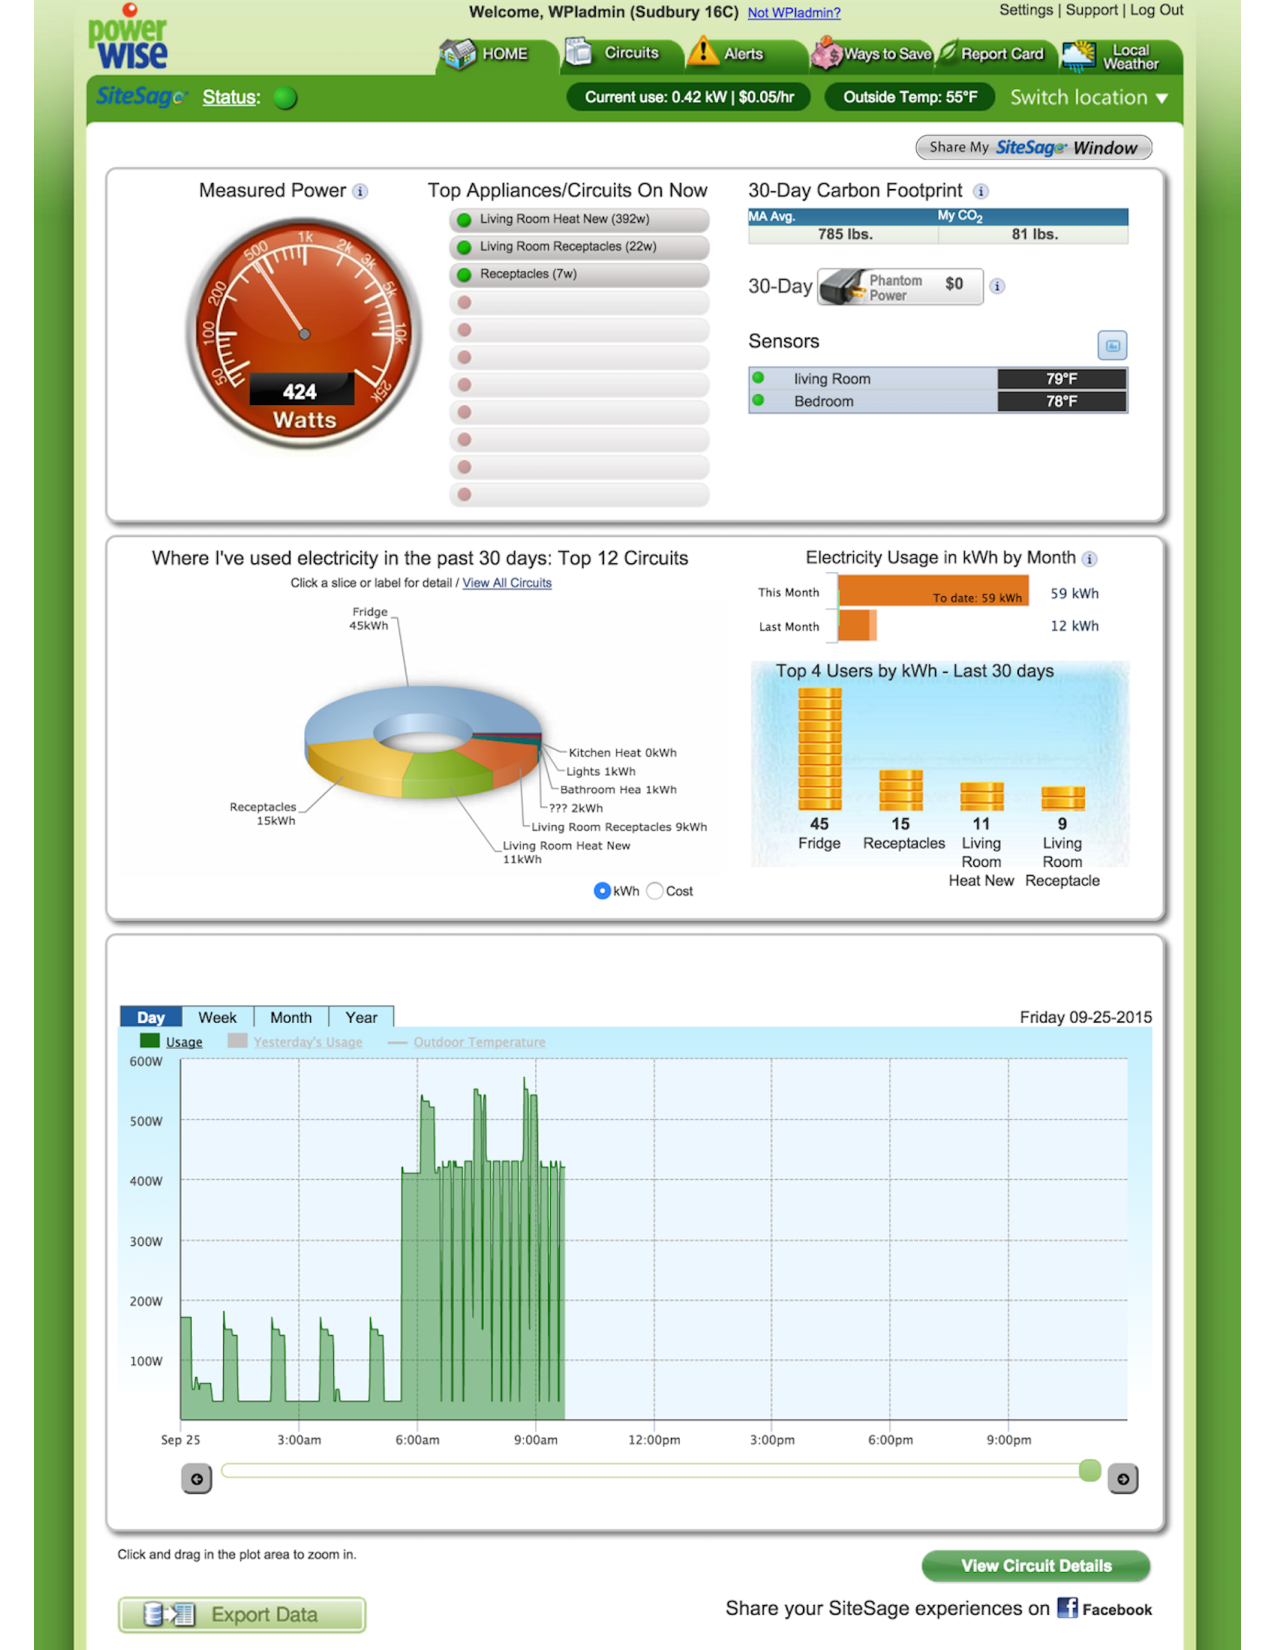
\includepdf{addins/powerwise.pdf}

\newpage
\section*{Appendix 2: Example Case Study}
\addcontentsline{toc}{section}{\numberline{}Appendix 2: Example Case Study}
\par Enclosed in this appendix is the example case study that was provided to us by the DOER. This case study acted as a guideline and template when we created case studies for the three project sites that we focused on.
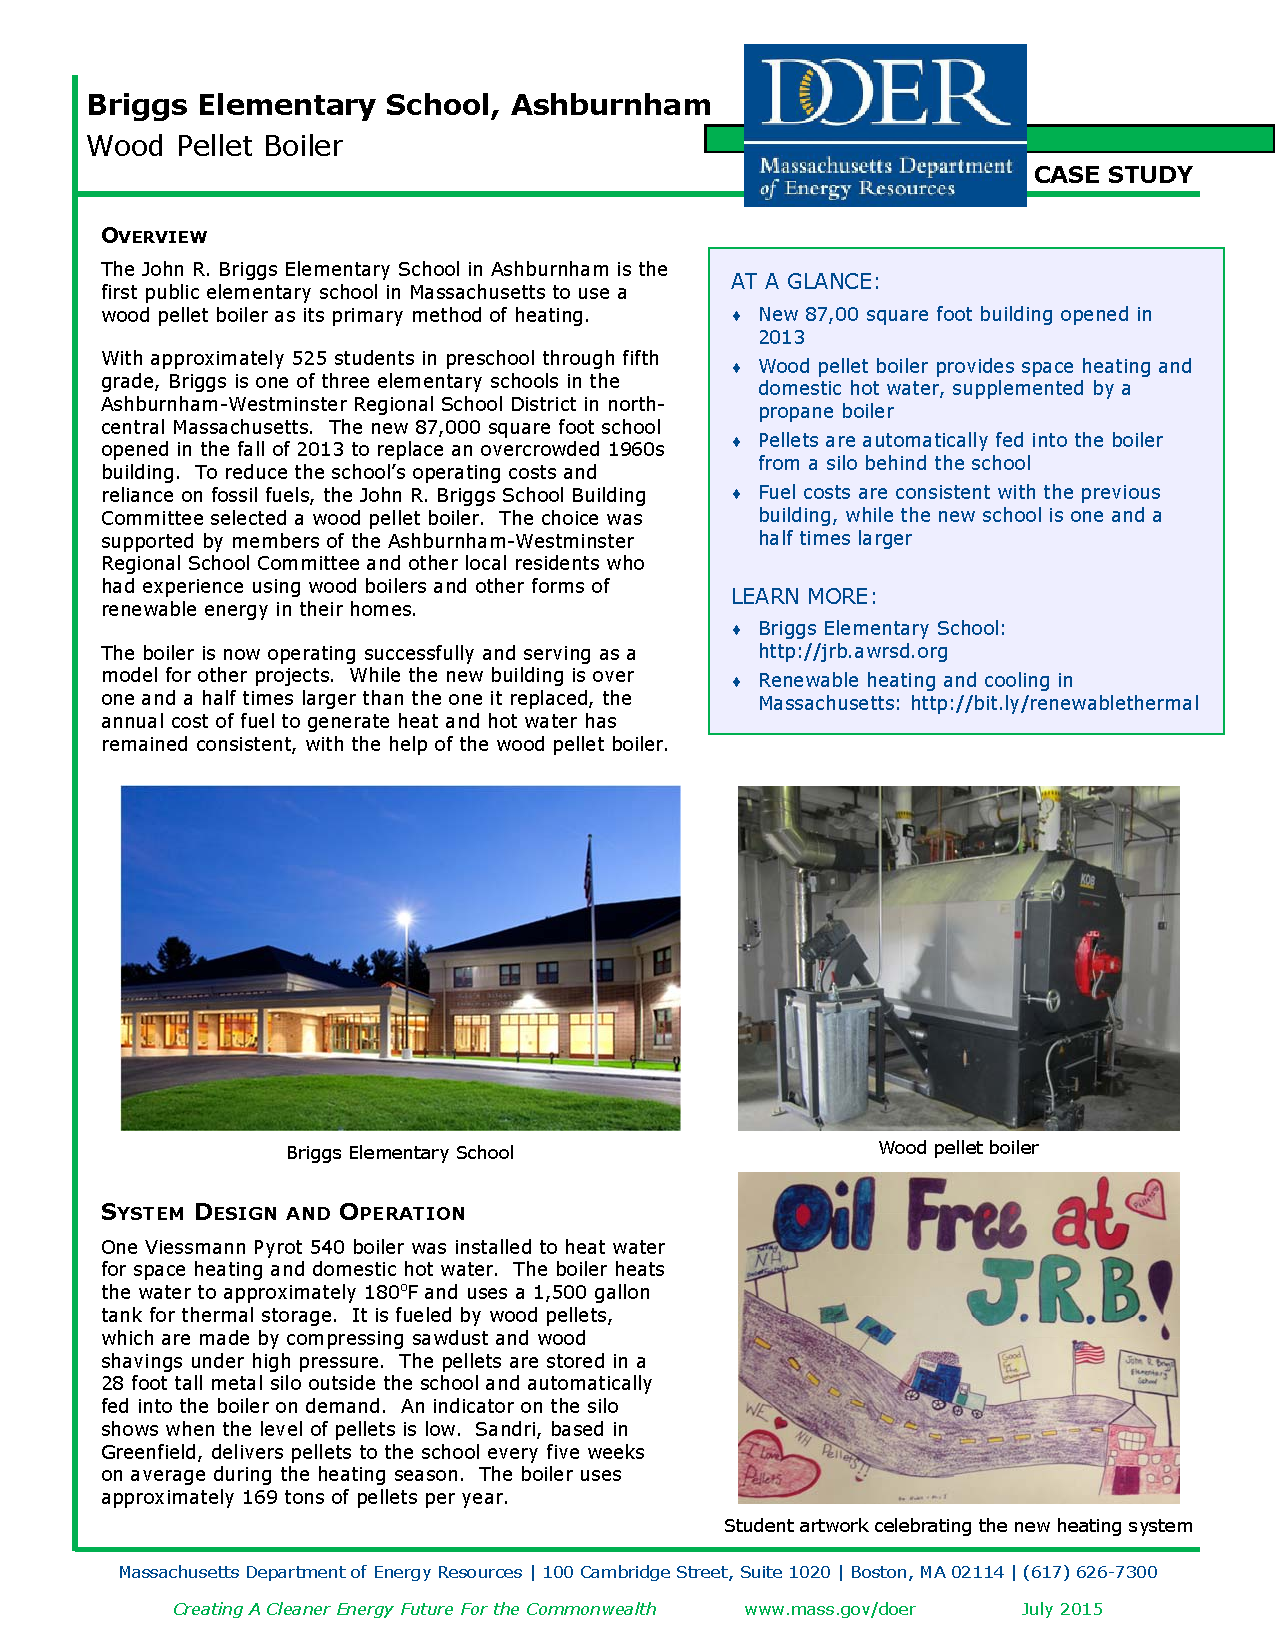
\includepdf[pages={1-}]{addins/briggs.pdf}

\newpage
\section*{Appendix 3: Interview Questions}
\addcontentsline{toc}{section}{\numberline{}Appendix 3: Interview Questions}
\par Below find the interview questions for each site along with the reasoning for asking each question. The interview questions are presented in the following order: Amherst College, Southern Berkshire Regional School, and Sudbury Public Housing Development.
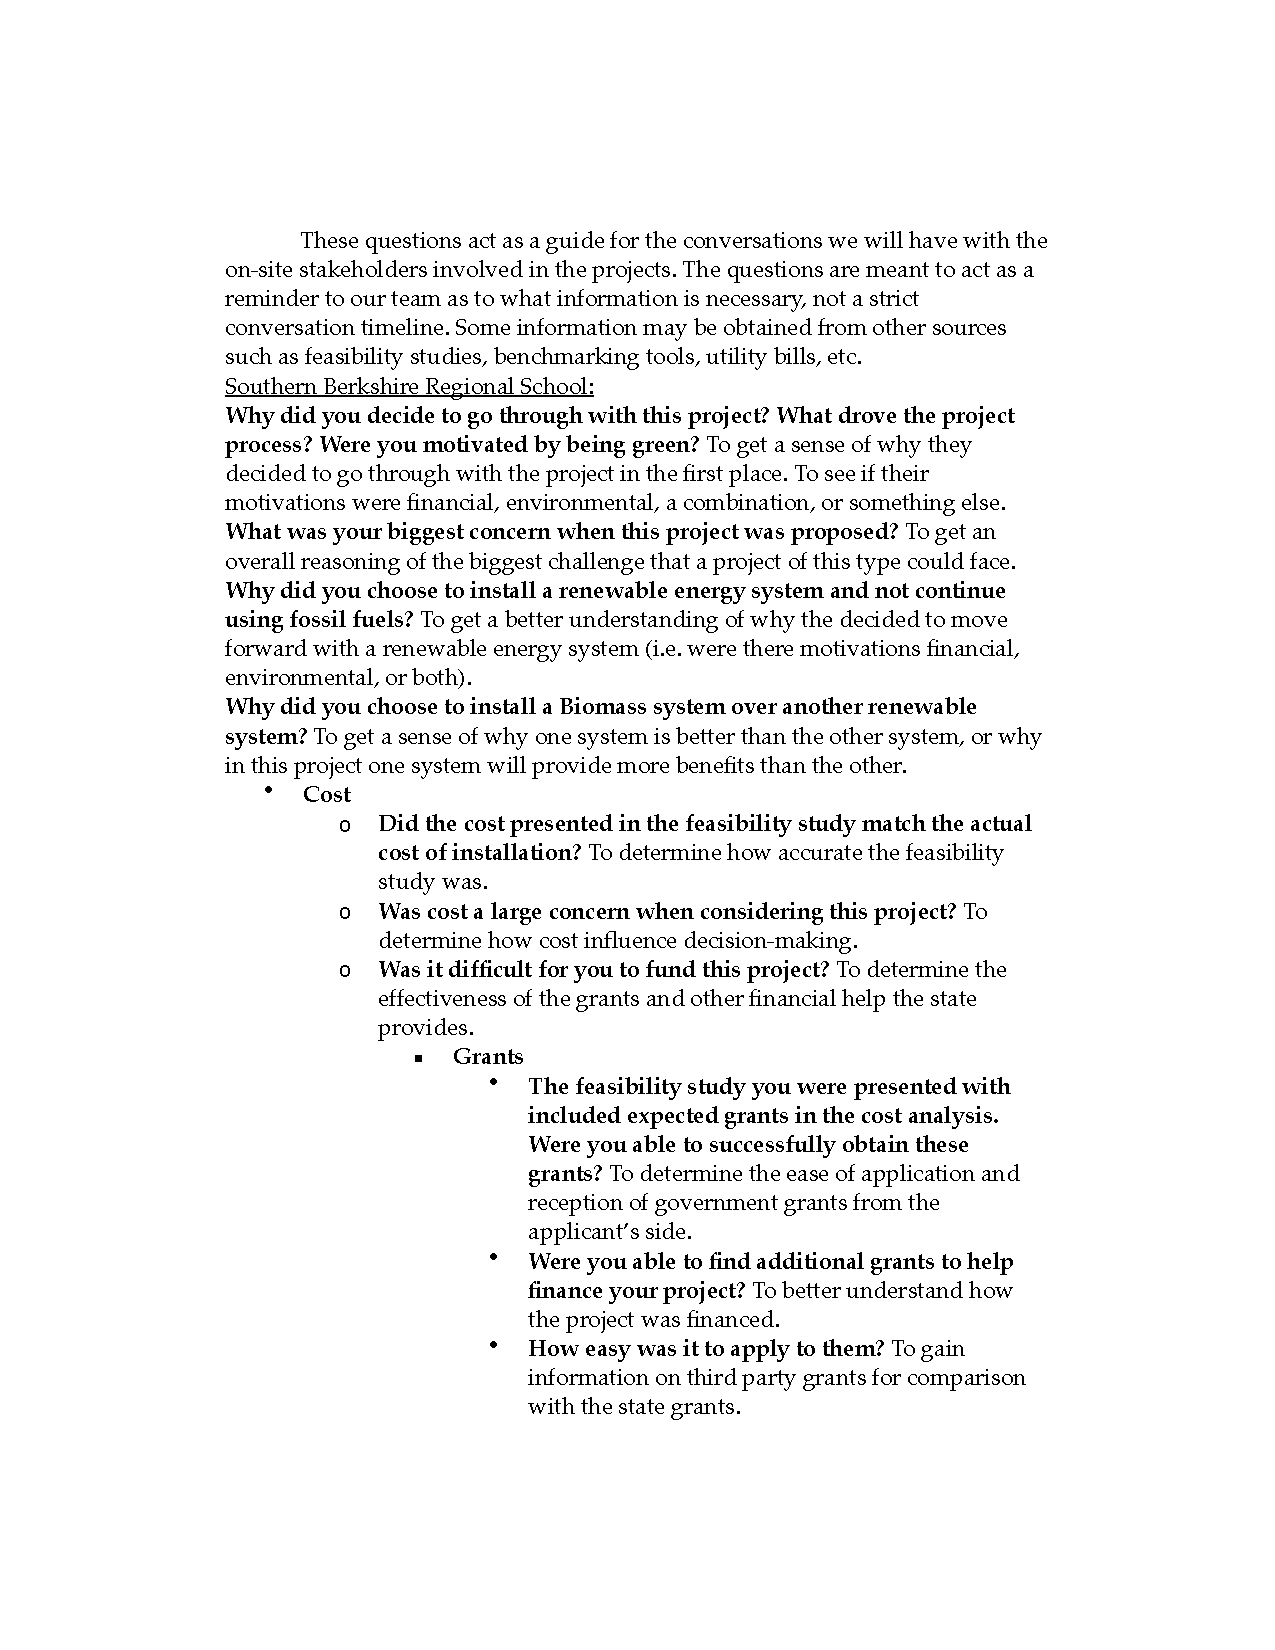
\includepdf[pages={1-}]{addins/app3.pdf}

\newpage
\section*{Appendix 4: On-site Information Gathering Guides}
\addcontentsline{toc}{section}{\numberline{}Appendix 4: On-site Information Gathering Guides}
\par The on-site information gathering guides for each site can be found below. Each site has its own gathering guide and included in each gathering guide is the information we had access to prior to our interviews. This information was obtained from feasibility studies of each site.
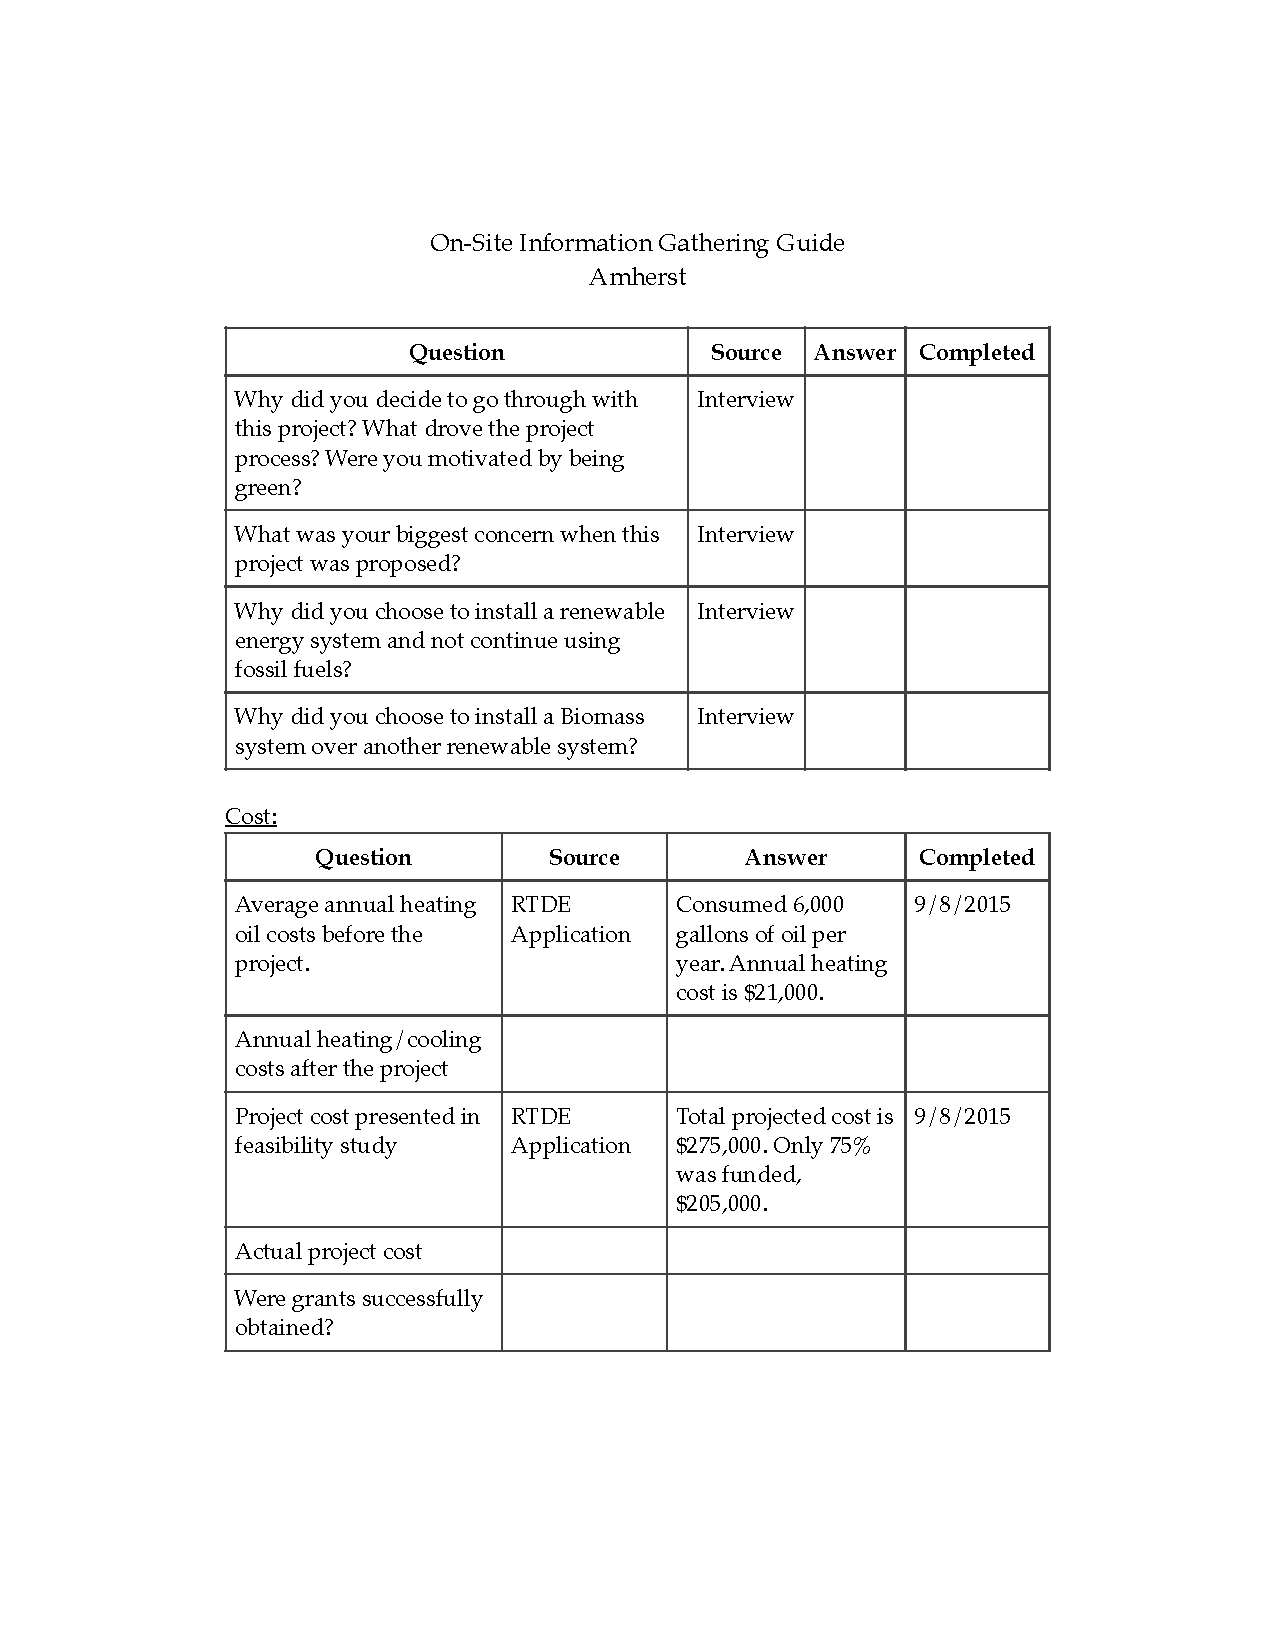
\includepdf[pages={1-}]{addins/app4.pdf}

\newpage
\section*{Appendix 5: Deliverables: Case Studies}
\addcontentsline{toc}{section}{\numberline{}Appendix 5: Deliverables: Case Studies}
\par Enclosed in this appendix are the case studies that we produced for the DOER as the project deliverables.
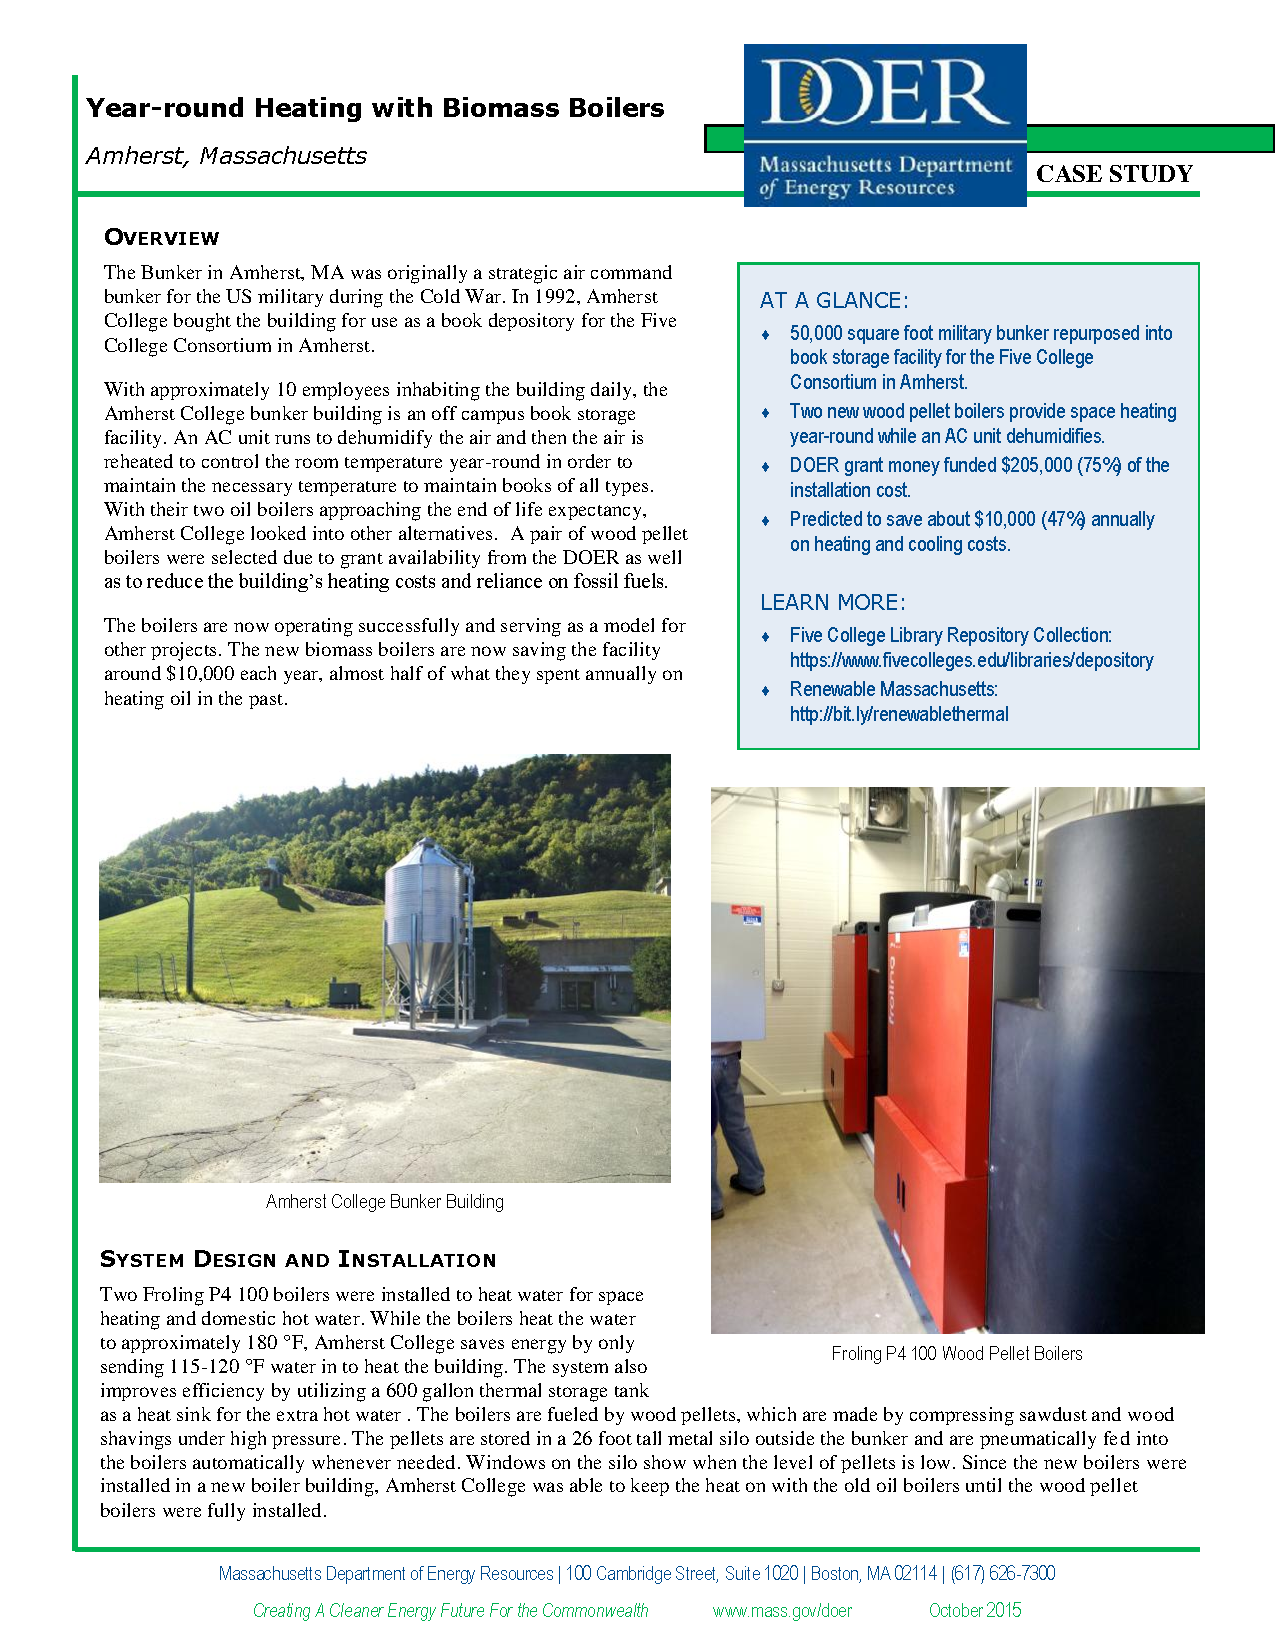
\includepdf[pages={1-}]{addins/amherst.pdf}
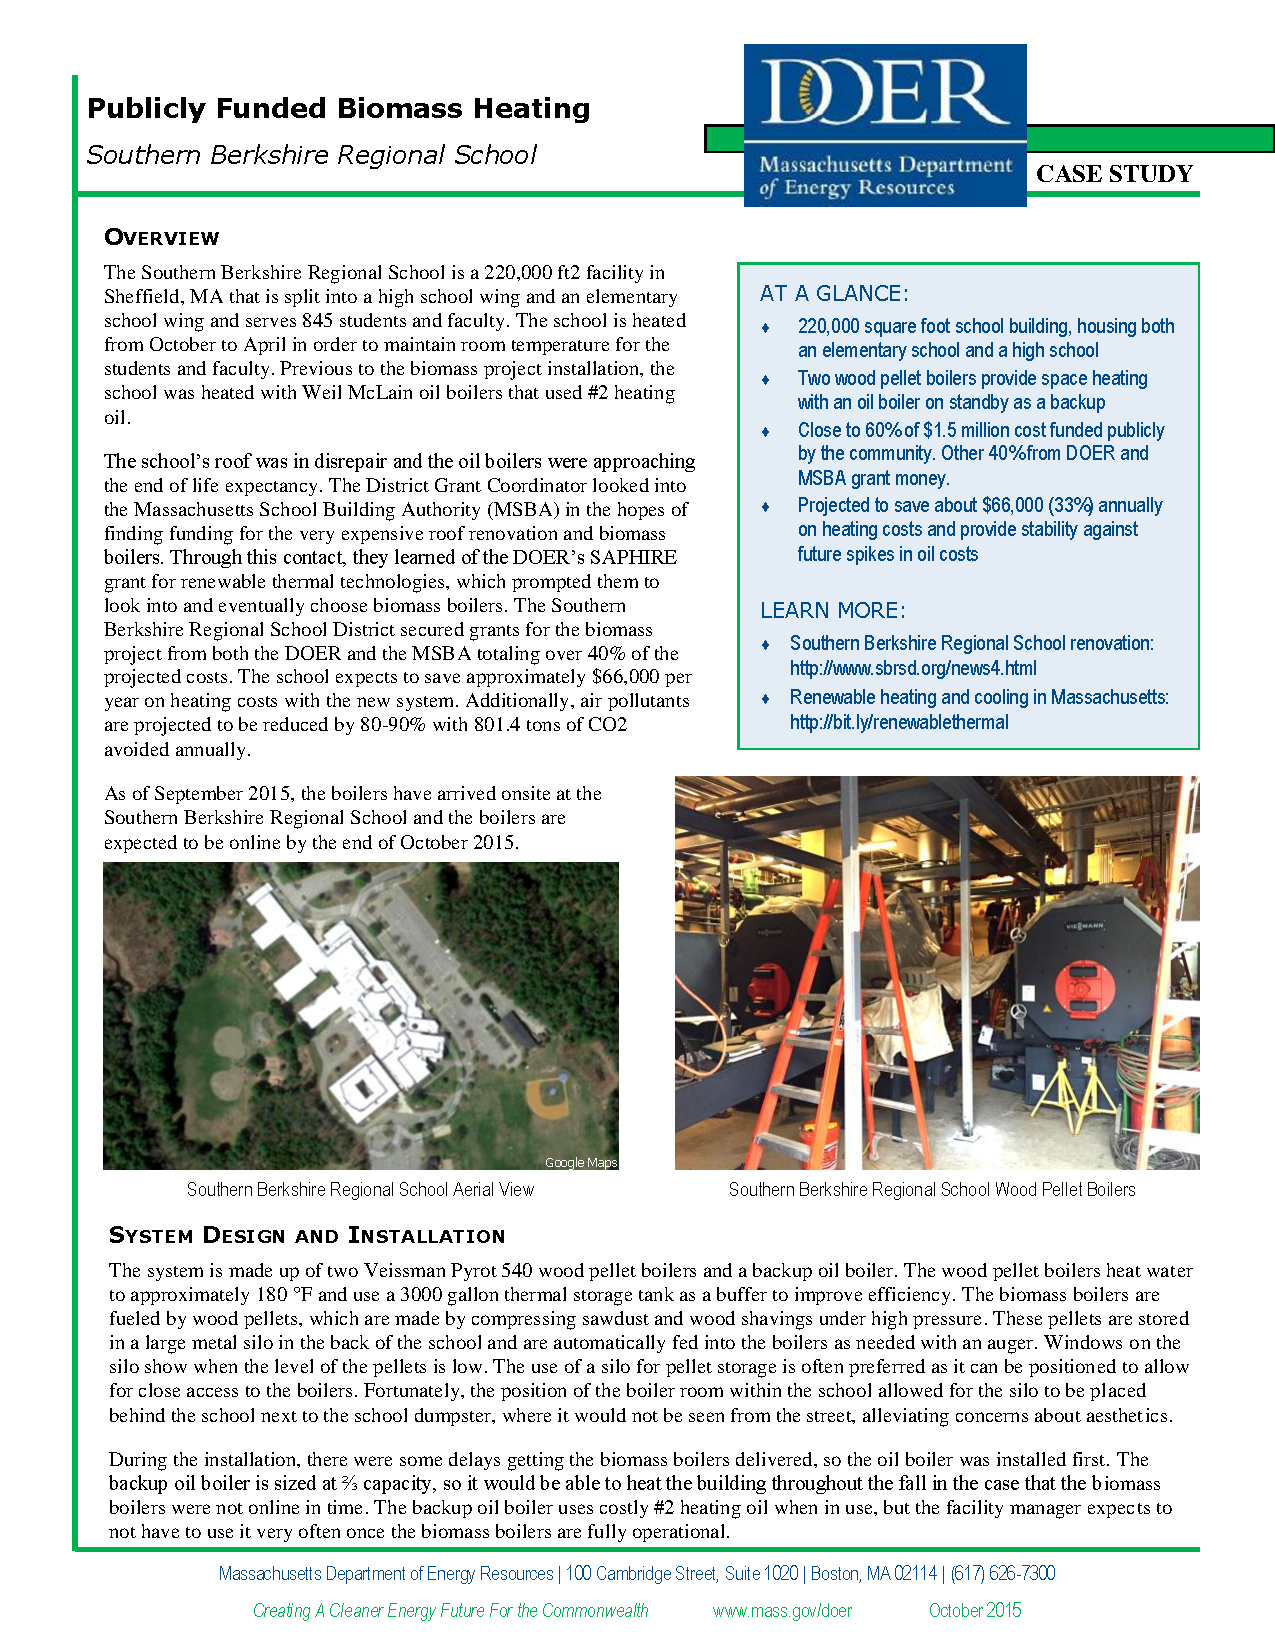
\includepdf[pages={1-}]{addins/sbrs.pdf}
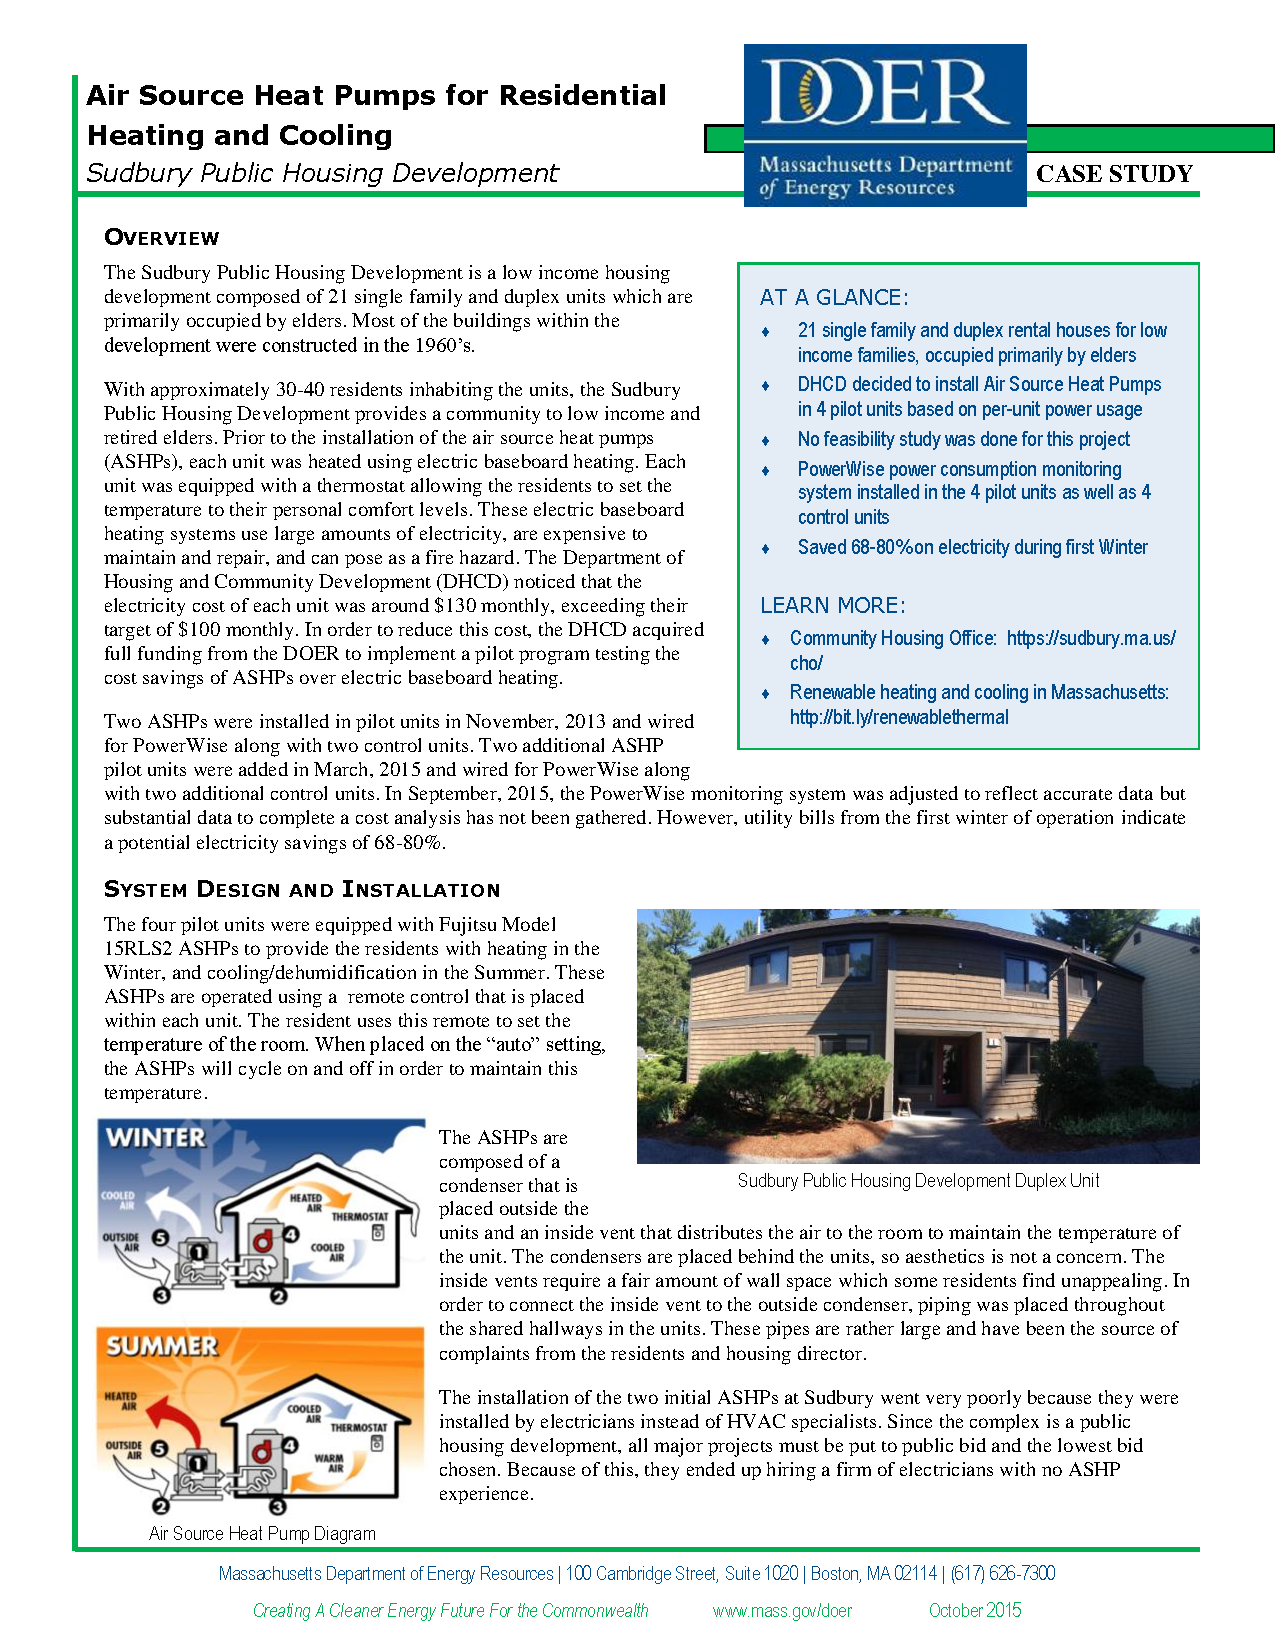
\includepdf[pages={1-}]{addins/sudbury.pdf}

\newpage
\section*{Appendix 6: Summative Assessment}
\addcontentsline{toc}{section}{\numberline{}Appendix 6: Summative Assessment}
\par Our team has worked very well together from the very beginning of our project. When we learned who our team members would be in ID 2050, we made an effort to get to know each other and become friends outside of the project. We accomplished this by doing activities together outside of class, like eating dinner. By becoming friends as well as teammates, we felt comfortable enough with each other to participate in open and honest conversations, as well as share honest comments and suggestions. Due to our strong bonds, we were easily able to resolve our few team conflicts and move forward with the project, producing a great result.
\par Our team's success is also due to specific strategies we utilized to bolster our productivity. At the beginning of the term we created a daily to-do list that we would continue to use throughout the term. We established a routine of using this to-do list to determine our tasks for the day. We would review the items on the list for the day on the train and assign team members to each item based on their strengths. In addition to the calendar and due dates provided by the project advisors, we made our own more detailed calendar with more specific due dates. This allowed us to internally stay on track and complete our assignments with enough time to allow for our site visits. Because we worked in separate cubicles at the DOER office, we used the chat feature of Google Documents to be communicate as we were writing or editing documents. 
\par Throughout the term, we split up the tasks to be done based on each team member's strengths and weaknesses. For example, Keirstan took the lead when interviewing stakeholders from each project site because she is comfortable with thinking on the fly due to past experience hosting radio shows. Another example is when producing the case studies for our sponsor, Jonas and Luis took the lead on writing the summaries and formatting each document because they are tech-savvy and more comfortable with compiling summaries than writing sections of the report. Keirstan and Carolina focused on writing and editing various sections of the report throughout the term because they have good writing skills and enjoy editing. Jonas did a lot of fine editing because he has the patience and grammatical knowledge to edit such a large report.
\par While we were already effectively accomplishing our work goals, after completing our formative assessments, we identified some areas for improvement within our team and applied corrective actions to remedy the situation. The first thing we noticed was that we were spending a lot of time writing sections of our paper. We quickly realized that this was because we were all writing at the same time. To remedy this situation we began splitting up the work based on each team member's strengths, and taking a moment at the end of the day to reconvene and discuss what had been accomplished that day. We also identified that there were some issues with time management and team members becoming distracted throughout the day. We took corrective action and had designated breaks from work in an effort to split up the day. We also removed all unnecessary distractions (i.e. phones, laptops) when collaborating on a single task. Finally, we identified that Keirstan was starting the conversation about what was to be completed each day. To remedy this, she allowed time for others to say their opinions and Jonas, Carolina, and Luis took initiative to provide their insights.
\par While we were able to improve our team's productivity by addressing several areas of concern, there is always room for each individual to grow into a better team member. For example, Keirstan seems to naturally fall into a leadership role. While this allows for increased productivity, sometimes every team member's opinions aren't heard. She plans on being more aware of the opinions of others within the group and allowing for others to step up into leadership roles. Jonas should take the initiative to do things beyond the baseline of what's on the schedule, which he will attempt to do on future projects. Carolina could try to rely less on the team for information that could be obtained from a different source. She will try to keep better track of emails and information relevant to the project. Luis plans to take more of a leadership role and express his opinions freely, instead of waiting for someone to delegate tasks for him to do.



